\documentclass[12pt]{article}
\usepackage{fullpage, times, epsfig}

%% For defining all text/page measurements. 170x240mm is the
%% standard thesis page size Ponsen & Looijen require. 124x185mm is
%% simply a text body size that resulted in margins that pleased me.
%% The dvips option will be superceded if pdflatex is used, but is
%% necessary in order to generate a correct PostScript bounding box
%% under standard LaTeX.

\usepackage[dvips]{geometry}

\newlength{\paperWidth}
%\setlength{\paperWidth}{5.605in}
\setlength{\paperWidth}{6in}
\newlength{\paperHeight}
\setlength{\paperHeight}{0.878\paperWidth}

% trim a bit more to reduce bottom whitespace
%\setlength{\paperHeight}{0.987\paperHeight}

\geometry{papersize={\paperWidth,\paperHeight},scale=1.0, vmargin={0in,0in}, headheight=0in, headsep=0in, footskip=0in}
%total={6.5in,5in}}


\begin{document}
\thispagestyle{empty}
{\noindent {\Huge About this Book}}\\
Exploring the collection of ``baby books'' at our local library, we noticed a striking absence of any mention or depiction of breastfeeding.
Our child, Mez, seemed particularly attracted to books with photographs, and we found plenty of pictures of babies eating solid foods (like chocolate, ice cream, and even {\it orange cheese curls}), but no images to which a breastfeeding baby or toddler could relate.
Breastfeeding is now recommended by experts across the board, so where are the baby books that depict it?
%Breastfeeding is no longer fringe, so where are the baby books that depict it?
We decided to create one.

%Rugged board books are ideal for babies and toddlers.
%However, they are quite labor-intensive to produce, with a lot of gluing and assembly.
%Thus, common publishing practice in 2005 seems to involving farming out the manufacturing to Asia to exploit cheap labor.
%Our only option was to self-publish and assemble the books ourselves.

The photographs for this book were shot on Saturday, September 4, 2004.
To fill gaps in the narrative, extra photographs were shot on Sunday, September 5, 2004.
The images were captured with a Sony DSC-F707 digital camera in 2560x1920 JPEG mode.
The images were converted to black-and-white using adjustment layers in Adobe Photoshop.
Each page was laid out using the illustration program Sketch (now called Skencil), which is free software.
The back page was typeset using \LaTeX, which is also free software. 

The pages of this book were printed by Rohrer Corporation in Wadsworth, Ohio.
This book was hand-assembled and bound with organic cotton in Potsdam, New York.

\begin{flushright}
\parbox{2in}{Lauren Serafin\\
Jason Rohrer\\
Potsdam, NY\\
October 2005}
\end{flushright}

\begin{center}
\fbox{
\begin{minipage}{.95\textwidth}
\noindent
\begin{minipage}{0.03\textwidth}
\begin{center}

\includegraphics[width=1em]{by_icon.eps}\\

\includegraphics[width=1em]{non_com_icon.eps}\\
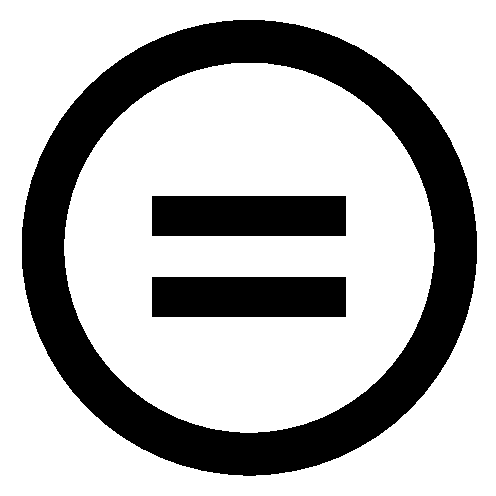
\includegraphics[width=1em]{no_derivs_icon.eps}
\end{center}
\end{minipage}
\begin{minipage}{0.97\textwidth}
This book is licensed under a Creative Commons {\em Attribution-NonCommercial-NoDerivs 2.5} License.
As long as you give us credit for our work, you can freely redistribute unmodified copies of this book for non-commercial purposes.\\
See http://creativecommons.org/licenses/by-nc-nd/2.5/
\end{minipage}
\begin{center}

\includegraphics[width=1in]{cc_logo.eps}
\end{center}
\end{minipage}
}
\end{center}


\end{document}



